\chapter{Development}\label{chap:devel}

This chapter will cover the architecture of the tool that was developed to
realise the objective of this thesis. This tool captures the paths that were
created, modified, and deleted in an \ac{IEEE} 802.11s mesh network, and
associates them with the packets that caused these events.

The tool consists of two programs: a program that captures the events and saves
them in output files, which will be referred to as \textbf{service}, and a
program to view the captured events of several computers side-by-side, referred
to as \textbf{central}. The way this tool is meant to be used is summarised in
\autoref{fig:usage}.

\begin{figure}[htb]
   \centering
   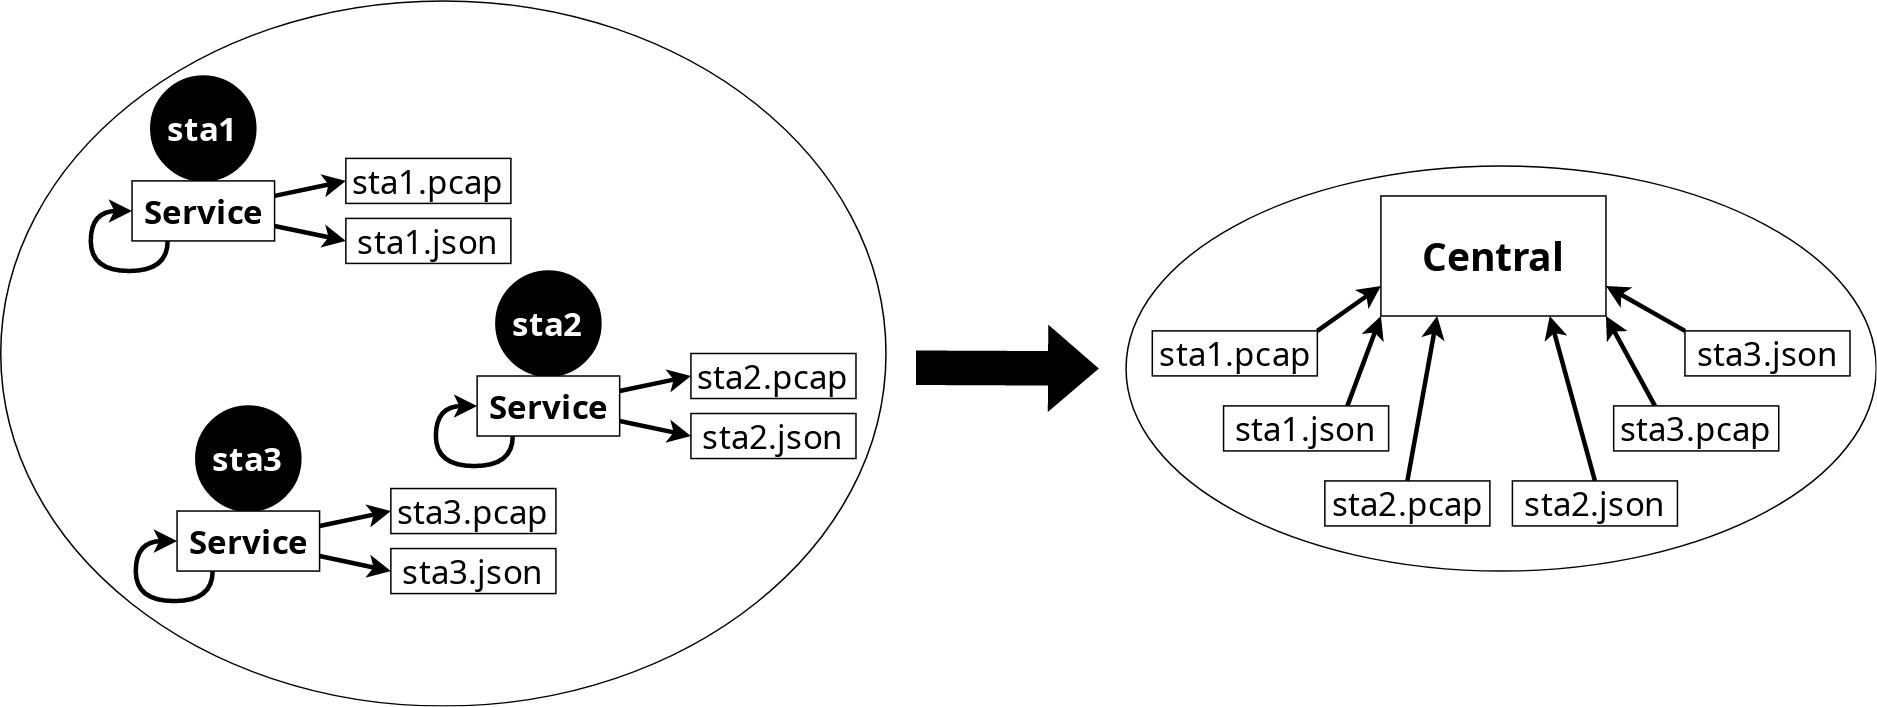
\includegraphics[scale=.225]{usage}
   \caption{Usage of the tool developed}\label{fig:usage}
\end{figure}


\section{Architecture of the Service}\label{sect:archser}

The \textbf{service} program can be divided into two parts. The eBPF part that
runs in the kernel-space and captures the events related to alterations in the
mesh path table, sending their details to user-space, and the Rust part that
runs in the user-space, receiving the data sent by the eBPF portion of the code,
while also capturing network packets at the same time in order to associate
packets to the actions performed in the system's mesh path table.

The \textbf{service} captures the events that alter the mesh path table and
network packets at the same time, saving them to output files, and when the user
sends a signal to stop, the program stops these captures. It starts by creating
the output files, a JSON file that stores a list of events and a network capture
file that stores packets, and then loads the eBPF code. Then, a new thread is
created whose sole purpose is to capture network packets. This new thread keeps
capturing packets and storing them in the appropriate output file in a loop that
only stops when the program receives a termination signal (one of
\texttt{SIGTERM}, \texttt{SIGQUIT}, or \texttt{SIGINT}).

Immediately after creating the packet capturing thread, the main thread goes
into a loop of its own doing the same thing, but instead of capturing packets,
it captures events sent by the eBPF code. This loop uses the same conditional
variable used by the packet capturing thread, so when one of the threads
receives a termination signal, both exit their respective loops.

After receiving a termination signal and leaving their loops, the packet
capturing thread stops, and the main thread continues. It then reads the
contents of both output files, creating a list of events and an iterator over
packets. The reason the program creates the output files at the start and writes
to them immediately, instead of creating these structures first and writing them
to the output files at the end, is to prevent the loss of data in case of a
crash, as well as to limit the memory usage of the program when it is run for a
long period of time.

With these two structures, the program goes over all the packets and events, and
checks which packets resulted in which events, storing this information in the
events themselves (this process is explained in more detail in
\autoref{subsec:relate}). Afterwards, it rewrites the output file for the
captured events with the newly modified events (including the packets each event
is related to), and terminates.


\subsection{eBPF Module}\label{subsec:ebpfcode}

The eBPF portion of the code is composed of nine probes. There are three probes
that detect if an alteration is made to the mesh path table, three to detect the
source of the action (if it was a packet reception or transmission that caused
the change in the mesh path table, or if it came from a command from
user-space), two for when a path is removed because it expired, and the last one
is for a special case which we will discuss later.

The three probes used to detect alterations in the mesh path table are in the
functions \texttt{mesh\_path\_add}, \texttt{mesh\_path\_assign\_nexthop}, and
\texttt{\_\_mesh\_path\_del}, the first two having been discussed in
\autoref{subs:mesh} and the last one in \autoref{subs:switch}. These are used to
gather information about the mesh path involved, including its destination,
nexthop, as well as the timestamp of the event and the MAC address and name of
the interface. The probe for \texttt{mesh\_path\_add} is the simplest, as it
only stores the information about the path that was added in a BPF map. In
another BPF map, the probe stores a value (which will be referred to as the
\textbf{situation} value) that indicates that the information stored in the
first BPF map came from a path addition to the mesh path table.
\autoref{fig:detai} shows in detail how this and the following probes use these
maps. The probe for \texttt{mesh\_path\_assign\_nexthop} is a bit more complex,
as this function is used both when a new path is added, and when an existing
path is altered, meaning that \texttt{mesh\_path\_add} can be called before it.
Because of this, this probe checks if there is a \textbf{situation} value
already present for the running thread in the BPF map, changing it to a new
value indicating if the situation is a new path being added or if it is an
existing path being modified. The information about the path is stored in the
appropriate BPF map if necessary. The relationship between these two probes can
be seen in \autoref{fig:addmod}. The last probe, in
\texttt{\_\_mesh\_path\_del}, detects the removal of paths from the mesh path
table, and if we ignore the possibility of paths being expired, it works just
like the probe for \texttt{mesh\_path\_add}. The case of a path being expired
will be explained shortly.

\begin{figure}[htb]
   \centering
   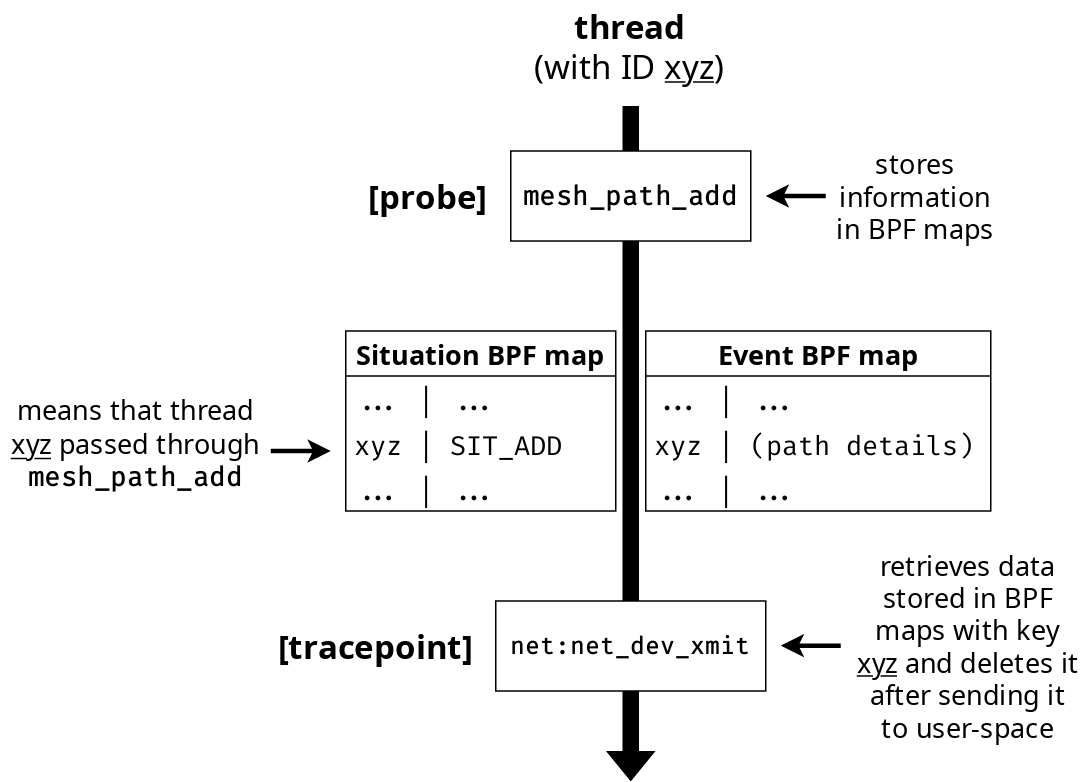
\includegraphics[scale=.375]{detail}
   \caption{Detail of BPF maps usage}\label{fig:detai}
\end{figure}

\begin{figure}[htb]
   \centering
   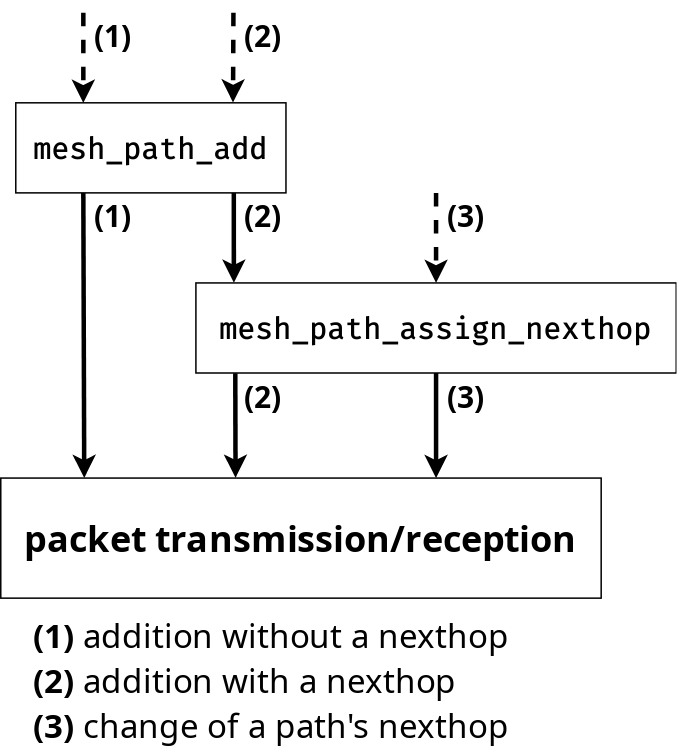
\includegraphics[scale=.35]{action}
   \caption{Probes for insertion and modification}\label{fig:addmod}
\end{figure}

For the next three probes, which are talked about in \autoref{subs:pkt}, two are
located in the tracepoints \texttt{net:net\_dev\_xmit} (packet transmission),
and \texttt{rdev\_return\_int} (command from user-space), and the third one is
in the function \texttt{ieee80211\_mesh\_rx\_queued\_mgmt} (packet reception).
These probes all work the same way. They take whatever is in the BPF maps, and
with the aid of the \textbf{situation} value, set the event's correct
\textbf{reason} field (which specifies the action taken on the mesh path table
and its source) and send the event to user-space to be received by the Rust
portion of the code, including the content of the link layer of the packet that
caused the event, if applicable.

There are also two probes at the entry and exit of the function
\texttt{mesh\_path\_expire}. The entry probe sets the \texttt{situation} value
in the proper BPF map, so that the probe at \texttt{\_\_mesh\_path\_del} sends
the event information directly to the user-space, while the exit probe simply
removes the data from the BPF maps, as it is not needed any more. The reason to
use two probes this way instead of having a single probe sending the data to
user-space directly (like the other three previously discussed), is because
\texttt{mesh\_path\_expire} calls \texttt{\_\_mesh\_path\_del} more than once.
Since only one event can be stored at a time per thread (because the threads'
IDs are being used as the keys in the BPF maps, and BPF maps do not allow the
usage of arrays of structures), only the information about the last path being
deleted would be sent to user-space instead of all paths. The way these probes
interact is demonstrated in \autoref{fig:delexp}.

\begin{figure}[htb]
   \centering
   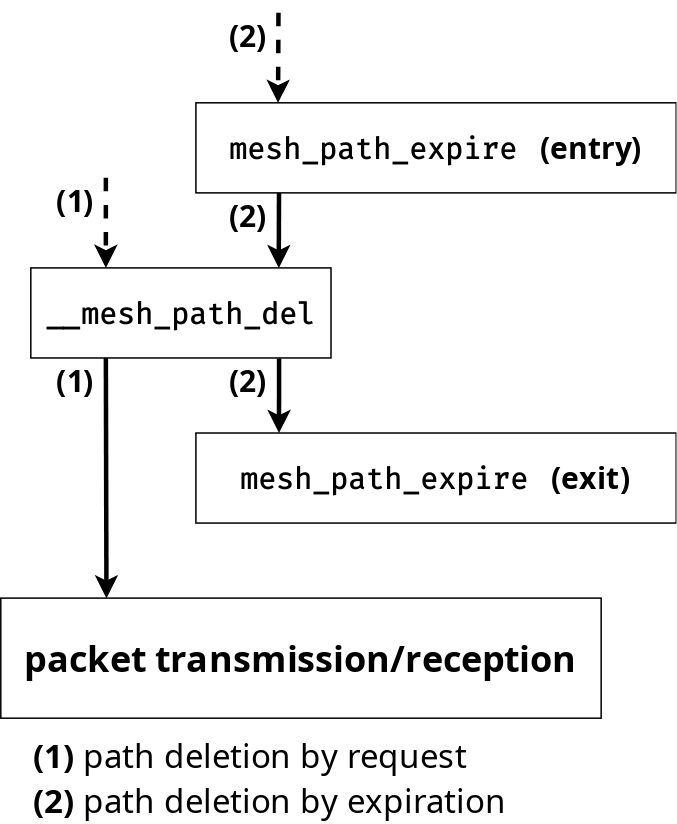
\includegraphics[scale=.35]{actiondel}
   \caption{Probes for deletion and expiration}\label{fig:delexp}
\end{figure}

Finally, there is also a probe in \texttt{mesh\_plink\_deactivate}, which is a
function that calls \texttt{\_\_mesh\_path\_del} indirectly. This probe is used
to ignore any calls to this function. The reason for this is that we were not
able to determine all the possible reasons for this function being called.
Packet transmission and reception would be captured, but some actions could be
missed. For example, we found that this function could be called by
\texttt{ieee80211\_sta\_expire}, and to capture this we would need more probes,
just like how probes for \texttt{mesh\_path\_expire} were required. Because we
found many functions calling \texttt{mesh\_plink\_deactivate}, and any of them
could end up requiring more probes, the time it would take to analyse all the
different possibilities would be too much, so we decided to ignore calls to this
function.


\subsection{Packet and Event Relation}\label{subsec:relate}

The packet/event relation section of the code is composed of two loops, one
inside the other. The program goes over every packet individually, and for each
one, it goes over every event that was captured. Even if an event gets matched
with a packet, the next packets will still check all events, including the ones
that matched with other packets earlier. This $O(n^2)$ algorithm is used, as
opposed to a more efficient one that would remove events as they are matched,
because of an issue that prevents us from obtaining the full content of a packet
in some events, where we have to ignore the missing content, which can lead to
an event matching more than one packet.

Because at the time of development a Rust library to access fields of network
packets did not exist, the program checks the raw data of the packets for the
fields manually in the array of bytes provided. It starts by making sure that
there are enough bytes to get all the data needed to compare with the details of
the event, and, if there are, compares the frame control, sequence control, and,
if applicable, \ac{QoS} control fields, as well as the address 1 and address 2
fields. As mentioned in \autoref{sect:mac802}, we noticed that in some events
the address 1 field obtained from the kernel-space was incorrect, it being the
address \texttt{00:00:00:00:00:00} instead of the expected value because the
computer that sends the packet does not know the \ac{MAC} address of the
receiver. We decided to ignore this field when it takes the aforementioned
value. We did not see this happen with the address 2 field, but do the same for
precaution.


\section{Architecture of the Central}\label{sect:archcen}

The \textbf{central} is a much simpler program than the \textbf{service}, as its
only goal is to display the events captured in a group of computers in a more
human-friendly way. Most of its code is for the \ac{GUI} logic.

The program takes a folder with the output files generated by the
\textbf{service} as an argument, and checks the file names, accepting only files
that end in \texttt{.json} and \texttt{.pcap}. For each pair of files that
contains the same stem, a structure called \texttt{Station} is created,
containing the list of events in the events file, and the name of the packet
capture file. After checking all files, a list of several \texttt{Station}
instances is returned.

The last step before displaying the events is to sort them in chronological
order. This is done by increasing the size of the list of events for each
station to have the capacity for all events in all the stations. Then, using
their timestamps, the events are ordered in such a way that, for each place in
the stations' lists, where one station has an event, all the others have an
empty element. This can be visualised in \autoref{fig:sort}. Although not very
efficient, it is the simplest method we could come up with to implement.

\begin{figure}[htb]
   \centering
   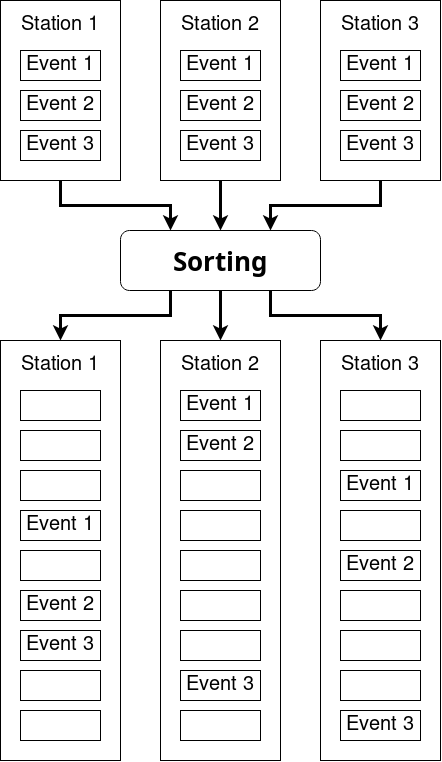
\includegraphics[scale=.4]{eventsort}
   \caption{Chronological sorting of events}\label{fig:sort}
\end{figure}

Finally, the \ac{GUI} is created, where the user can view all the events of all
the stations side by side, and not only inspect the details of each event, but
also see the packets that caused those events in Wireshark with the press of a
button. \autoref{fig:hardtest} displays an example capture.

\begin{figure}[htb]
   \centering
   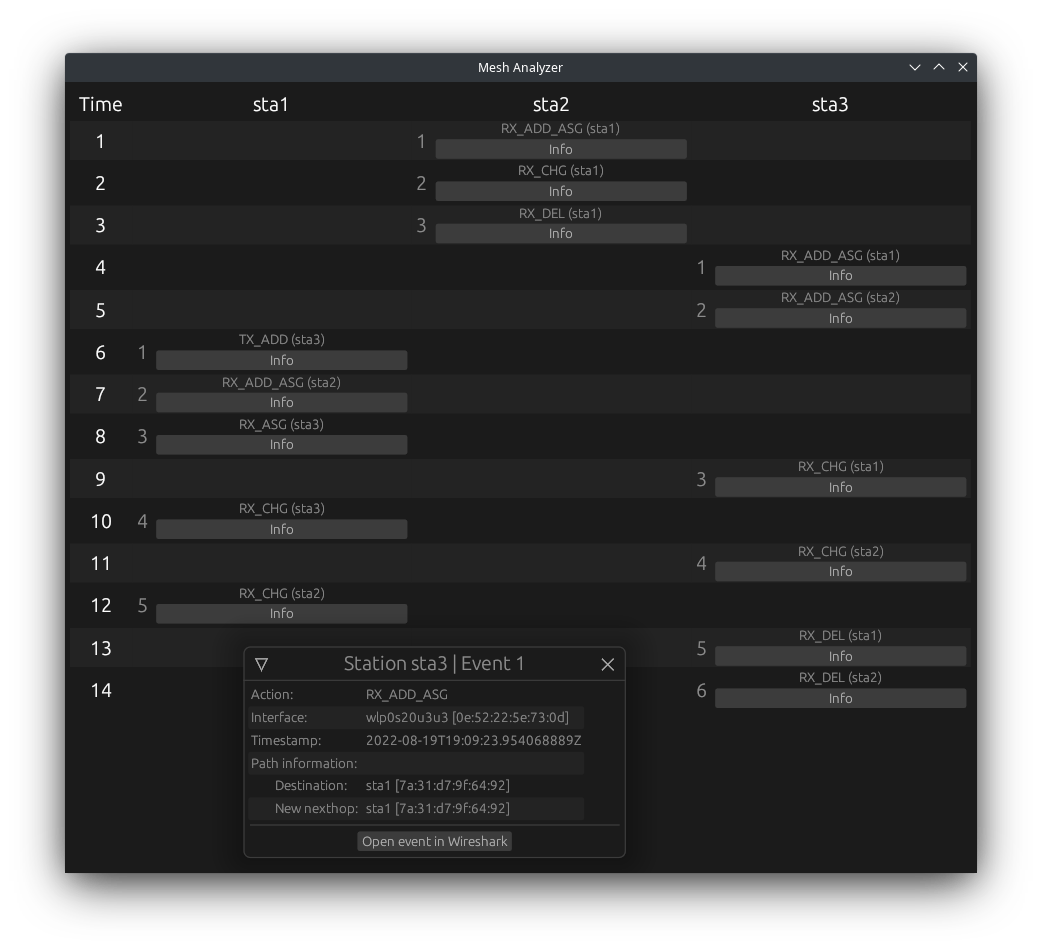
\includegraphics[scale=.575]{gui}
   \caption{\ac{GUI} interface}\label{fig:hardtest}
\end{figure}
